\begin{enunciado}
 Las calificaciones de un curso de estad\'{\i}stica para un semestre
 espec\'{\i}fico fueron las siguientes:
 \begin{center}
  \begin{tabular}{l|cccc}
   Calificaci\'on & A & B & C & D \\
   \hline
   $f$ & $14$ & $18$ & $32$ & $20$
  \end{tabular}
 \end{center}
 Pruebe la hip\'otesis, al nivel de significancia de $0.05$,
 de que la distribuci\'on de calificaciones es uniforme.
\end{enunciado}

\begin{solucion}
 Para la soluci\'on, se define la variable aleatoria $X$
 como una codificaci\'on de las calificaciones.
 As\'{\i}, $X=1$ indica la calificaci\'on A; $X=2$, la calificaci\'on B;
 $X=3$, la calificaci\'on C; y, $X=4$, la calificaci\'on D.
 \begin{datos}
  $\phantom{0}$
  \begin{itemize}
   \item Tama\~no de la muestra: $n=14+18+32+20=84$.
   \item Frecuencias observadas:
   $O = = \{ o_1 = 14, o_2 = 18, o_3 = 32, o_4 = 20 \}$.
   \item Probabilidades esperadas: $p_i = f(i;4)$,
   la funci\'on de probabilidad uniforme discreta con par\'ametro $k=4$,
   es decir $p_i = \frac{1}{4}, \forall i \in \mathbb{N}\cap[1,4]$.
   \item frecuencias esperadas:
   $E = \left\{ \left. e_i = n\cdot p_i = \frac{84}{4} = 21 \, \right| \, \forall i \in \mathbb{N}\cap[1,4] \right\}$.
   \item Celdas totales del experimento: $k=4$.
   \item Grados de libertad de la prueba $\chi^2$: $v = k-1 = 3$.
  \end{itemize}
 \end{datos}

 \begin{hipotesis}
  Prueba de bondad de ajuste para probar $H_0:$
  que una variable aleatoria $X$ sigue una distribuci\'on uniforme
  $f(x;k) = f(x;4)$, para $x\in\mathbb{N}\cap[1,4]$
  contra la alternativa $H_1$ de que no es as\'{\i}.
 \end{hipotesis}

 \begin{significancia}
  $\alpha = 0.05$.
 \end{significancia}

 \begin{region}
  De la tabla A.5 se tiene el valor cr\'{\i}tico
  $\chi^2_{\alpha,v} = \chi^2_{0.05,3} = 7.815$,
  por lo que la regi\'on de rechazo est\'a dado
  para $\chi^2 > 7.815$, donde
  $\chi^2 = \sum_{i=1}^k \frac{\left( o_i - e_i \right)^2}{e_i}$.
 \end{region}

 \begin{estadistico}
  \begin{eqnarray*}
   \chi^2 & = & \sum_{i=1}^k \frac{\left( o_i - e_i \right)^2}{e_i}
   =\frac{(14 - 21)^2}{21} + \frac{(18 - 21)^2}{21} +
   \frac{(32 - 21)^2}{21} + \frac{(20 - 21)^2}{21} \\
   & = & \frac{7^2 + 3^2 + 11^2 + 1^2}{21} = \frac{180}{21}
   = \frac{60}{7} = 8.\overline{571428}
  \end{eqnarray*}
 \end{estadistico}

 \begin{decision}
  Se rechaza $H_0$ a favor de $H_1$.
 \end{decision}

 \begin{conclusion}
  Hay suficiente evidencia para afirmar que las calificaciones
  no siguen una distribuci\'on uniforme.
 \end{conclusion}

 Finalmente, usando el archivo anexo
 \texttt{P15\_Prueba\_de\_bondad\_chi2\_01.r},
 que a su vez requiere los datos del archivo
 \texttt{DB18\_Problema\_082.csv}, con los siguientes cambios:
 \begin{verbatim}
> datos<-read.csv("DB18_Problema_082.csv",sep=";",encoding="UTF-8")
> varInteres<-"Frecuencia"
> varCelda<-"Calificaciones.puntaje"
> distribucion<-1
> parametro_nombre<-NULL
> parametro_valor<-NULL
> combinar<-TRUE
> grafica<-TRUE
> tituloEjeX<-"Calificaciones del curso de Estadística"
> alfa<-0.05
 \end{verbatim}
 \vspace{-0.5cm}
 el programa de R lanza el siguiente resultado:
 \begin{verbatim}
                Variable Distribución de ajuste Estadístico Chisq2
1 Calificaciones.puntaje               Uniforme           8.571429
  Grados de libertad    Valor-p alpha Región de Rechazo
1                  3 0.03556654  0.05       > 7.8147279
                       Resultado
1 Se rechaza el ajuste de bondad
 \end{verbatim}
 \vspace{-0.5cm}
 que incluye la siguiente figura:
 \begin{center}
  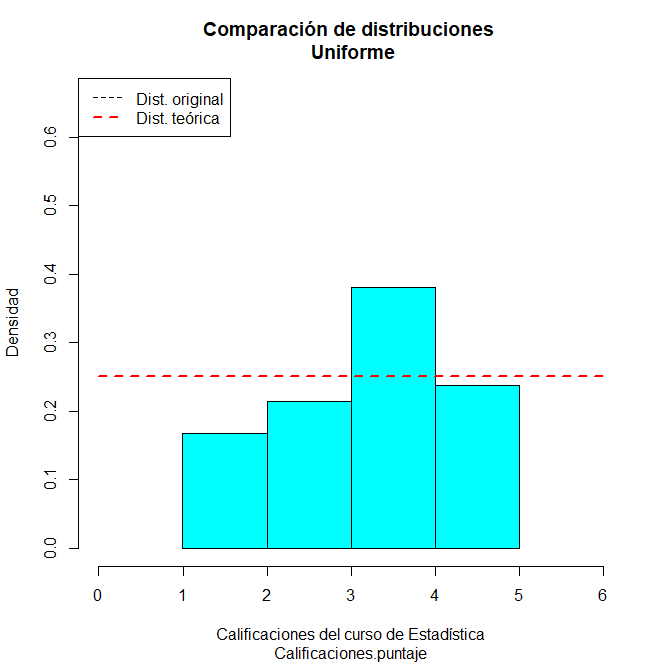
\includegraphics[scale=0.4]{Problema_82.png}
 \end{center}
 El cual coincide con los datos obtenidos,
 que es a lo que se quer\'{\i}a llegar.${}_{\blacksquare}$
\end{solucion}
